\section{Stolpersteine}

Es wird davon ausgegangen, dass sich mit der Variation von $k_{max}$ bei der 
Welle keine grossen Ver"anderungen einstellen. Die Werte werden immer ab einem 
gewissen Punkt ins Positive oder Negative explodieren, da das $x^k$ irgendwann 
dominiert. Mit $k_{max}$ wird die Anzahl der Summanden bezeichnet, die f"ur die 
Berechnung der Potenzreihe verwendet werden. 

\begin{equation*}
y(x) = a_0 + a_1x 
-\sum_{k=2}^{k_{max}}\frac{1}{k(k-1)}(aa_{k-4}+ba_{k-3}+ca_{k-2})x^k
\end{equation*}

Es werden die Startbedingungen gem"ass den Gleichungen 
\ref{wellen:Startbedingungen1} festgelegt.

\begin{equation}
	\begin{split}
		a_0 &= 1\\
		a_1 &= 0\\
		a &= 1\\
		b &= 0\\
		c &= -1
	\end{split}
	\label{wellen:Startbedingungen1}
\end{equation}

Auf folgenden Grafiken wird veranschaulicht, was mit der Welle passiert, wenn 
das $k_{max}$ jeweils um 30 vergr"ossert wird. Es wird dann "uberpr"uft, ob 
sich die Behauptung der kleinen Ver"anderungen als wahr herausstellt.

\begin{center}
	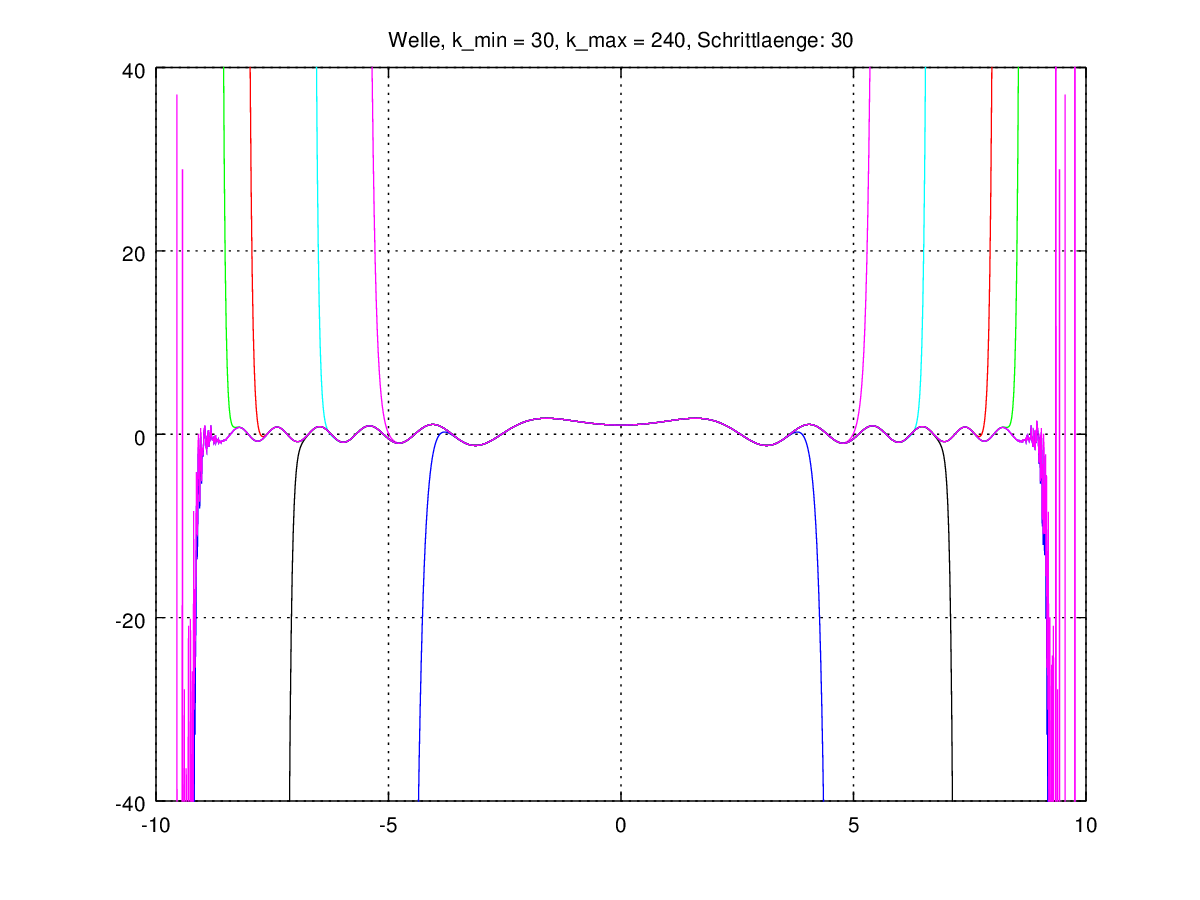
\includegraphics[scale=0.69]{./wellen/images/kmax/krangewaveeven.png}
\end{center}

Die Behauptung, dass der Wert irgendwann explodiert, ist, wie ersichtlich, 
wahr. Der Punkt wo die Werte gegen $\infty$ gehen verschiebt sich immer mehr 
nach rechts, zu gr"osseren $x$-Werten. Dies wird dadurch erkl"art, dass es 
immer l"anger geht, bis der $x^k$-Term dominiert. Je mehr der $k_{max}$-Wert 
gesteigert wird, umso besser wird die Approximation an die Welle. Ab einer 
gewissen Gr"osse von $k_{max}$ kann das Programm die Werte nicht mehr genau 
bestimmen, was die unregelm"assigen Ausschl"age erkl"art.

Aufgrund dieser Messungen wird $x$ f"ur die weiteren Berechnungen auf $x \in 
[-8;8]$ und $k_{max}$ auf 180 beschr"ankt, damit die $y$-Werte nicht 
explodieren und keine unkontrollierten Messwerte entstehen.

Mit den in diesem Kapitel festgelegten Startbedingungen und Einschr"ankungen 
ergibt dies folgende Grafik:
\begin{center}
	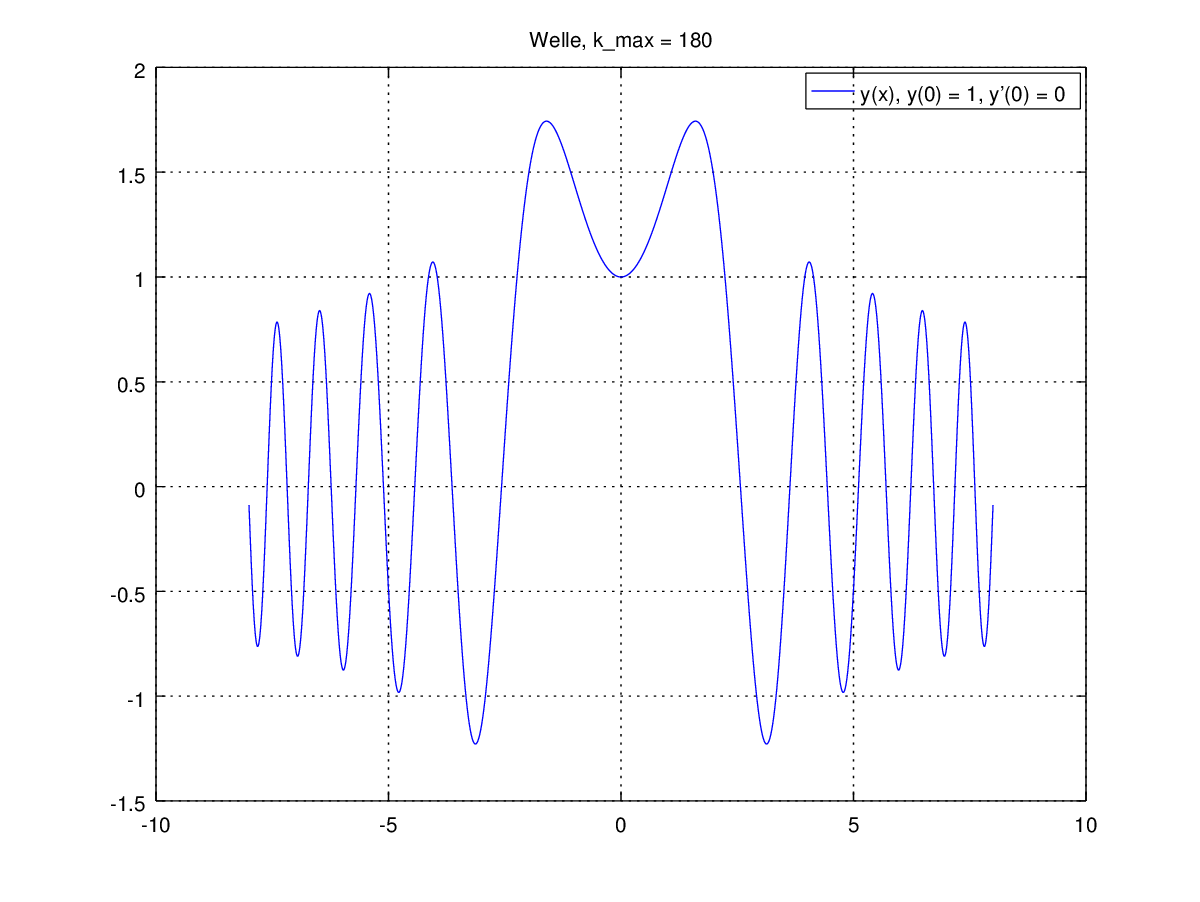
\includegraphics[scale=0.69]{./wellen/images/kmax/ak180-88wave.png}
\end{center}

